% --- Documentclass specifications ---
\documentclass[italian]{tktltiki2}
\linespread{1.3}

% --- General packages ---
\usepackage[utf8]{inputenc}
\usepackage[T1]{fontenc}
\usepackage{lmodern}
\usepackage{epigraph}
\usepackage{microtype}
\usepackage{amsfonts,amsmath,amssymb,amsthm,booktabs,color,enumitem,graphicx}
\usepackage[pdftex,hidelinks]{hyperref}
% setting C language style listing
\usepackage{listings}
\lstset{
  language=C,
  basicstyle=\fontsize{8}{11}\selectfont\ttfamily
}
% Automatically set the PDF metadata fields
\makeatletter
\AtBeginDocument{\hypersetup{pdftitle = {\@title}, pdfauthor = {\@author}}}
\makeatother

% --- Language-related settings ---
\usepackage[fixlanguage]{babelbib}
% add bibliography to the table of contents
\usepackage[nottoc]{tocbibind}


% --- tktltiki2 options ---
%
% The following commands define the information used to generate title and
% abstract pages. The following entries should be always specified:
\title{%
    \huge Project Heimdall 
    \\
    \large Proposta di implementazione per un web switch 
    \\ 
    concorrente two-way di livello 7 (OSI) con 
    \\
    politiche di bilanciamento del carico stateless e stateful
  }
  \author{\emph{Alessio Moretti} - 0187698
    \\
    \emph{Andrea Cerra} - 0167043
    \\
    \emph{Claudio Pastorini} - 0186256}
  \date{\today}
  \level{Corso di Ingegneria di Internet e del Web - A.A. 2014/2015}
  \university{\textbf{Università degli studi di Roma Tor Vergata}}
  \department{\textbf{Facoltà di Ingegneria Informatica}}
  \city{Roma}

\begin{document}

% --- Front matter ---
\maketitle        % title page

\tableofcontents  % table of contents
\pagenumbering{gobble}

% --- Main matter ---
\mainmatter       % clear page, start arabic page numbering

\section{Example section}
% Example of a quote
\begin{quote}
\flushright
	\emph{Yggdrasil, l'albero del mondo, che congiunge i nove regni del cosmo con Asgard, la dimora degli dei.} 
  \\
  Heimdall, custode del Bifröst
\end{quote}

% Write some science here
Sample text and a reference\cite{lamport94}. Lorem ipsum dolor sit amet, consectetur adipiscing elit. Donec at lorem varius, sodales diam semper, congue dui. Integer porttitor felis eu tempor tempor. Proin molestie maximus augue in facilisis. Phasellus eros dui, blandit eu nibh ut, pharetra porta enim. Cum sociis natoque penatibus et magnis dis parturient montes, nascetur ridiculus mus. Aliquam ullamcorper risus pretium est elementum, eget egestas lorem fermentum. Etiam auctor nisi purus, vitae scelerisque augue vehicula sed. Ut eu laoreet ex. Mauris eu mi a tortor gravida cursus eget sit amet ligula.

\begin{figure}
\centering

\includegraphics[width=\textwidth]{images/thor}
\caption{Thor di Asgard, \emph{figlio di Odino}}
\end{figure}

\newpage
\section{Introduzione}
\subsection{Perché Heimdall?}
Heimdall è il personaggio dell'universo Marvel, ispirato all'omonimo dio della mitologia norrena, egli è il guardiano del regno di Asgard e del Bifröst. Quest'ultimo è il ponte che unisce la Terra alla dimora degli dei ed Heimdall, come suo custode, ha il compito di aprirlo ed indirizzarlo verso gli altri mondi, permettendo solamente a chi è degno di attraversare le distese dello spazio.
\\
Ci piace pensare che questo sia un po' il ruolo del software nato dal nostro progetto: che sia in grado di scegliere come meglio indirizzare le connessioni in arrivo, ponendosi come ``guardiano'' di un cluster di server che fa ad esso capo. Quindi un \textbf{web switch} che sia funzionale sia per ricevere o trasmettere pacchetti di un regolare traffico HTTP, che per bilanciare il carico dello stesso traffico in arrivo sulle varie macchine.

\subsection{Web switch di livello 7}
Nella terminologia delle reti informatiche uno \textbf{switch} è un commutatore a livello datalink, ovvero un dispositivo che si occupa di instradare opportunamente, attraverso le reti LAN, selezionando i frame ricevuti e reindirizzandoli verso la macchina appropriata a seconda di una propria tabella di inoltro. Un \textbf{web switch}, a livello applicativo, è capace di reindirizzare i dati in funzione dei pacchetti che riceve, analizzandone il contenuto e decidendo opportunamente la destinazione, occupandosi allo stesso tempo di reinoltrare anche l'eventuale risposta della macchina selezionata verso il client che l'ha generata.
\\
Le applicazioni sono molteplici per l'implementazione a livello applicativo: può essere considerato un \textbf{proxy}, oppure, selezionando opportunamente la macchina con più velocità di risposta o con minore pressione, può agire come \textbf{bilanciatore di carico}. Infatti ognuno dei client che fa richiesta, ad esempio, per uno specifico sito web, invia un pacchetto ad un indirizzo IP pubblico che corrisponde a quello del nostro switch applicativo. Questi, dopo aver correttamente letto il pacchetto, si occupa di consultare una tabella di inoltro generata con una determinata \textbf{politica di scheduling} e quindi gestire l'inoltro della richiesta ed il reinoltro della risposta del webserver. Tutto questo in maniera totalmente trasparente al client, qualsiasi sia la macchina che ha effettivamente risposto, che sia un web server oppure un cluster di macchine associate ad un ulteriore switch.

\subsection{Assunzioni progettuali sul cluster}
Nella fase di progettazione e realizzazione sono state definite le seguenti assunzioni:
\begin{itemize}
	\item Ognuna delle macchine del cluster dispone di un web server Apache in ascolto sulla porta 80
	\item Ognuna delle macchine monta il modulo ApacheStatus come monitor di carico
\end{itemize}


\begin{figure}
\centering
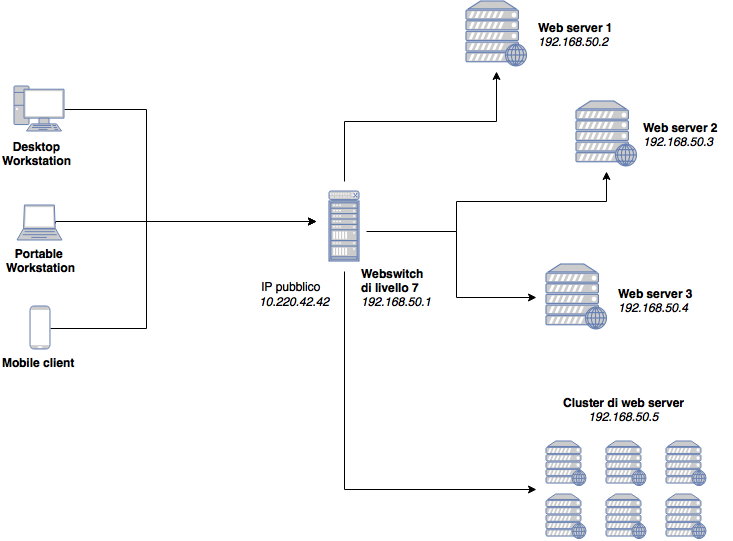
\includegraphics[width=\textwidth]{images/switch7}
\caption{Esempio di uno \emph{switch di livello 7 (OSI)}}
\end{figure}

\newpage
\section{Architettura}
\label{sec:architecture}

\subsection{Overview}
\label{ssec:overview}

\subsection{Server in ascolto}
\label{sec:main}

\subsection{File di configurazione}
\label{sec:config}
I file di configurazione sono gli unici file accessibili all'utente che installa sulla propria macchina Heimdall WebSwitch. Tramite questi file è possibile impostare alcuni parametri per adattare il WebSwitch alle proprie esigenze.\\\\
I file di cui stiamo parlando sono due e adesso ne illustreremo i dettagli.
\subsubsection{File dei parametri}
\label{sec:config_parser}
Questo è il file di configurazione generale di Heimdall. Al suo interno possiamo trovare i seguenti parametri:

\begin{itemize}
	
	% TODO modificare quelle macro con descrizioni decenti e mettere ref
	\item \emph{algorithm\_selection}: specifica il tipo di algoritmo che si vuole usare per Heimdall, con il valore 0 si sceglie di usare l'algoritmo STATELESSRR, con il valore 1 si sceglie di usare l'algoritmo STATEFUL.
	
	% TODO ref a worker per i processi figli
	\item \emph{pre\_fork}: specifica il numero di proessi figli che verranno creati all'avvio di Heimdall, i processi figli ricordiamo sono i processi che gestiranno le connessioni HTTP. Se il valore di questo parametro viene impostato a 0 Heimdall creerà automaticamente 1 processo figlio per gestire le richieste.
	
	\item \emph{print\_enable}: abilita le stampe a video se impostato a 1, altrimenti le disabilita.
		
	\item \emph{log\_level}: specifica il livello di stampe che si vogliono avere sul terminale, i livelli di log saranno spiegati bene nella sezione dedicata.
	
	\item \emph{write\_enable}: abilita la scrittura dei file di log.
 	
	\item \emph{log\_file\_req}: specifica il percorso del file di log per le connessioni richieste a heimdall.
		
	\item \emph{log\_file\_resp}: specifica il percorso del file di log per le risposte fatte alle connessioni.
		
	% TODO spiegato meglio nella sezione del watchdog?
	\item \emph{timeout\_worker}: specifica il	
	\item \emph{update\_time}: questo parametro indica il
	
	\item \emph{server\_config} specifica il percorso del file di configurazione dovengono specificati i server del cluster collegati a Heimdall.
	
	\item \emph{server\_main\_port}: specifica la porta di ascolto del processo padre di Heimdall per accettare nuove connessioni.
			
	\item \emph{backlog}: specifica il valore di backlog passato alla funzione accept.
	
	\item \emph{max\_fd}: specifica il numero massimo di connessioni persistenti che Heimdall è in grado di gestire. Questo parametro può variare in base al numero massimo di file descriptor che possono essere contemporaneamente aperti nel sistema.
	
	\item \emph{sockets\_path}: specifica una directory del sistema dove Heimdall potrà creare socket AF\_UNIX, necessarie per permettere la comunicazione tra il processo padre e i suoi figli. Heimdall dovrà avere permessi di lettura e scrittura su questa directory.
	
	\item \emph{max\_thread\_pchild}: specifica il numero massimo di thread\_request che ogni Worker può creare, e cioè il massimo numero di richieste che possono essere accettate contemporaneamente su una singola connessione persistente.
	
\end{itemize}
Rappresentiamo qui con un esempio un file dei parametri:

\begin{lstlisting}
	# STATELESSRR 0 STATEFUL 1
	algorithm_selection 1

	# The number of active processes to handle requests
	# If prefork is 0, the system create anyway 1 child process
	pre_fork 10

	# If 1 log print to shell is enabled
	print_enable 1

	# Specify the log level desired
	log_level 2

	# Write on log file enabled, see log_file_req and log_file_resp variable
	write_enable 0
	
	...
	...
	
\end{lstlisting}

\subsubsection{File dei server}
\label{ssec:config_server}
Il file dei server è il file dove vengono specificati i server del cluster collegati a Heimdall, questo file è specificato (all'interno del file di configurazione) nel parametro \emph{server\_config}. Al suo interno vengono specificati un nome per il server associato ed il relativo indirizzo ip.
\\\\Rappresentiamo qui con un esempio un file dei server:

\begin{lstlisting}

# Server 1
Name:bifrost.asgard
IP:192.168.1.4

\end{lstlisting}

\subsubsection{Implementazione dei file di configurazione}
\label{ssec:file_config_impl}

La lettura del file dei parametri spetta al parser Heimdall Config, la sua implementazione è presente nei file heimdall\_config.c e heimdall\_config.h \\\\ All'interno del file .h sono presenti alcuni valori necessari al funzionamento del parser, tra questi troviamo:

\begin{itemize}

\item Una costante \emph{CONFIGFILE} dove va specificato il percorso del file dei parametri.
	
\begin{lstlisting}
/*
 * ---------------------------------------------------------------------------
 * Relative position to config file
 * ---------------------------------------------------------------------------
 */
#define CONFIGFILE "../code/config/heimdall_config.conf"
\end{lstlisting}
	
\item Una struttura dati di tipo \emph{ConfigPtr}

\begin{lstlisting}
/*
 * ---------------------------------------------------------------------------
 * Structure        : Config struct
 * Description      : This struct collect all config value from config file.
 * ---------------------------------------------------------------------------
 */
typedef struct config{
    char *algorithm_selection;
    char *pre_fork;
    char *print_enable;
    char *log_level;
    char *write_enable;
    char *log_file_req;
    char *log_file_resp;
    char *timeout_worker;
    char *killer_time;
    char *update_time;
    char *server_config;
    char *server_main_port;
    char *backlog;
    char *max_fd;
    char *sockets_path;
    char *max_thread_pchild;
} Config, *ConfigPtr;	
\end{lstlisting}

\end{itemize}
Come possiamo notare i campi della struttura sono esattamente le chiavi che abbiamo elencato precedentemente nel paragrafo relativo al file dei parametri. Come si vede dall'esempio i campi all'interno del file sono disposti in un ordine preciso, dettato da una regola ti tipo \emph{chiave:valore}. Il parser esegue la lettura del file una riga per volta, estrae la chiave, il suo valore e passa il tutto ad una funzione di callback.

\begin{lstlisting}
/*
 * ---------------------------------------------------------------------------
 * Function     : _get
 * Description  : Used for get key and value from a line.
 *
 * Param        :
 *   array[]    : line string.
 *   from       : from value start.
 *   to         : escape character where function stop.
 *
 * Return       : string.
 * ---------------------------------------------------------------------------
 */
char *_get(char array[], int from, char escape){

    int from_cpy = from;
    int total = 0;

    while (1) {
        if (array[from_cpy] == escape)
            break;
        ++from_cpy;
        ++total;
    }

    total++; // add \0 space

    char *subset = malloc(sizeof(char) * total);    
    if (subset == NULL) {
        fprintf(stderr, "Error in _get config_parser. \n");
        return NULL;
    }

    int j;
    for(j = 0; j < total - 1; ++j, ++from) {
        subset[j] = array[from];
    }

    subset[total-1] = '\0';

    return subset;
}

/*
 * ---------------------------------------------------------------------------
 * Function     : init_config
 * Description  : Parse config file and call callback function for return values.
 *
 * Param            :
 *   path           : Path to file be parsed.
 *   config_handler : Callback function, return to main key, value and config reference.
 *   ptr_config     : Pointer to struct.
 *
 * Return       :
 * ---------------------------------------------------------------------------
 */
int init_config(const char *path, int config_handler(char *key, char *value, void *p_config), void *ptr_config) {

    singleton_config = ptr_config;

    // open file
    FILE *config_file = fopen(path, "r");
    if (config_file == NULL) {
        fprintf(stderr, "Error while trying to open config file. \n");
        return -1;
    }

    // while each line
    char string[MAX_LENGTH];

    while(fgets(string, MAX_LENGTH, config_file)) {

        // skip, line comment or empty line
        if (string[0] == '#' || string[0] == '\n')
            continue;
        
        char *key = _get(string, 0, ESCAPE_CHARACTER);
        if (key == NULL) {
            fprintf(stderr, "Error in init_config config_parser. \n");
            return -1;
        }

        char *value = _get(string, strlen(key)+1, '\n');
        if (value == NULL) {
            fprintf(stderr, "Error in init_config config_parser. \n");
            return -1;
        }

        if(config_handler(key, value, ptr_config) == -1) {
            fprintf(stderr, "Error config parser, no key '%s' found in Config. \n", key);
            return -1;
        }

        free(value);
        free(key);
    }

    fclose(config_file);

    return 0;
}
\end{lstlisting}
La funzione config\_handler riceve la chiave e il valore estratto, ed effettuando un semplice confronto con la chiave esegue l'inserimento del valore all'interno della struct.

\begin{lstlisting}
/*
* ---------------------------------------------------------------------------
* Function     : config_handler
* Description  : Callback function, see heimdall_config.c for more information.
*
* Return       : 0 if ok, -1 if error.
* ---------------------------------------------------------------------------
*/
int config_handler(char *key, char *value, void *p_config) {

    Config* config = (Config *)p_config;
        
    if (strcmp(key, "algorithm_selection") == 0) {
        if (asprintf(&config->algorithm_selection, "%s", value) == -1)
            return -1;

    }else if (strcmp(key, "pre_fork") == 0) {
        if (asprintf(&config->pre_fork, "%s", value) == -1)
            return -1;
            
            ...
            ...
            
    }else
        return -1;  /* unknown key, error */

    return 0;
}
\end{lstlisting}
Il funzionamento del parser per il file dei server è a grandi linee lo stesso, il codice relativo può essere trovato nei file server\_config.c e server\_config.h. Unica differenza è che questo parser non ritorna una struct con tutti i valori del file config bensì ritorna una struttura contenente questi valori:

\begin{lstlisting}
/*
 * ---------------------------------------------------------------------------
 * Structure        : Config struct
 * Description      : This struct collect all config value from config file.
 * ---------------------------------------------------------------------------
 */
typedef struct server_config{
    char **servers_names;
    char **servers_ip;
    int total_server;
} ServerConfig, *ServerConfigPtr;
\end{lstlisting}
Ossia un array di puntatori ai nomi, un array di puntatori ai relativi indirizzi ip e un intero che indica il numero totale dei server identificati nel file, quest'ultimo utile per scansionare gli array descritti.
\\\\Come ultima caratteristica di implementazione facciamo notare che la lettura dei file e quindi la relativa esecuzione dei parser viene eseguita solamente una volta all'avvio del programma, questo per ridurre gli evidenti accessi di I/O che sarebbero necessari per estrarre di volta in volta il valore richiesto. Per fare ciò è stato quindi utilizzato un approccio alla programmazione chiamato \emph{Singeleton}, infatti una volta eseguito il parser dei file, il riferimento alla struttura viene salvato nella variabile globale:

\begin{lstlisting}
/*
 * ---------------------------------------------------------------------------
 * Description  : Global variable, singleton instance of Config
 * ---------------------------------------------------------------------------
 */
void *singleton_config = NULL;
\end{lstlisting}
Un semplice controllo viene comunque eseguito ed è lo stesso controllo che avvia l'esecuzione del parser la prima volta, se la variabile è NULL viene eseguita la lettura del file ed inizializzata la relativa struttura. Grazie poi alla chiamata fork() che viene eseguita qualche momento dopo tutti i figli riceveranno "gratuitamente" in eredità la struttura Config.

\subsection{Logging}
\label{sec:logging}

\subsection{Gestione degli errori}
\label{sec:errors}

\subsection{Pool manager}
\label{sec:pool}

\subsection{Scheduler} 
\label{ssec: sched}
Lo scheduler è un componente fondamentale di un sistema informatica: si occupa di stabilire un ordinamento temporale l'esecuzione di un set di richieste di accesso ad una risorsa. Nel caso di un web switch di livello 7, lo scheduler va a garantire che ognuna delle richieste in arrivo possa essere inoltrata immediatamente alla prima macchina disponibile, secondo una politica di scheduling che sia \emph{state-less}, quindi che non consideri l'attuale carico di lavoro delle macchine del cluster, oppure \emph{state-aware}, che monitori costantemente tale carico e modifichi di conseguenza l'assegnazione delle richieste (verrà spiegato nel dettaglio come lavorano e quando sono disponibili tali politiche in \emph{\ref{sec: sched_p}}). \\\\
In questa implementazione lo scheduler, che come vedremo va a sfruttare un algoritmo di selezione \emph{Round Robin} la cui struttura verrà esplicitata più avanti, viene definito come segue.
\begin{lstlisting}
/*
 * ---------------------------------------------------------------------------
 * Structure        : typedef struct scheduler_args
 * Description      : This struct represents the arguments necessary to run the
 *                    scheduler properly
 * ---------------------------------------------------------------------------
 */
typedef struct scheduler_args {
    RRobinPtr     rrobin;                                   // Round Robin struct
    ServerPoolPtr server_pool;                              // Server Pool struct

    ServerPtr (*get_server)(RRobinPtr rrobin);              // to retrieve a server
} Scheduler, *SchedulerPtr;


\end{lstlisting}
In particolare la \textbf{pool dei server} altro non è che un \emph{lista collegata} formata da strutture dati elementari per la gestione dei server indicati nel file di configurazione come appartenenti al cluster, definite come segue
\begin{lstlisting}
/* ---------------------------------------------------------------------------
 * Structure        : typedef struct server_node
 * Description      : This struct represents a single server node in order to
 *                    manage a pool of remote machines
 * ---------------------------------------------------------------------------
 */
typedef struct server_node {
    char *host_address;                                         // machine canonical name
    char *host_ip;                                              // machine ip address
    int  status;                                                // machine status
    int  weight;                                                // machine weight

    struct server_node *next;                                   // next server_node
} ServerNode, *ServerNodePtr;

\end{lstlisting}
mentre le strutture dati che vengono elaborate ed utilizzate come valore di ritorno della schedulazione e che sono alla base della costituzione del buffer su cui opera Round Robin, non sono altro che una versione semplificata e costituita dalle sole informazioni di base per la connessione. \\\\
Nella \textbf{fase di inizializzazione} viene quindi popolata la pool recuperando gli indirizzi delle macchine del cluster, che vengono settate come disponibili e con peso minimo. Quindi a seconda che si sia configurato il web switch in modalità \emph{state-aware} o \emph{state-less}, rispettivamente viene o non viene istanziato un thread che si occuperà di aggiornare periodicamente, con gestione degli accessi concorrenti al buffer del Round Robin, lo stato delle macchine. Ogni volta che una connessione viene accettata viene recuperato un server valido da passare al processo che gestirà la connessione tramite memoria condivisa.
\begin{lstlisting}
\* inside thread pool ... *\
// Retrieving server from scheduler
ServerPtr server = get_scheduler()->get_server(get_scheduler()->rrobin);
// Storing server in shared memory
worker_pool->worker_server[position] = *server;
	
\end{lstlisting}
Viene sempre selezionato un server che sia disponibile, quindi viene sempre effettuato un controllo sullo \emph{status} dello stesso server, nel caso in cui sia abilitato il controllo sullo stato della macchina: l'unico caso in cui questi risulta \emph{BROKEN} e non \emph{READY} è nella circostanza in cui ogni server del cluster risulta non disponibile per cui il worker (che analizzeremo in \emph{\ref{sec:worker}}) non avvierà nessuna connessione di inoltro della richiesta. \\\\
Dalla necessità progettuale di garantire uno \textbf{scheduling adattabile} a condizioni di stress da carico, quindi per soddisfare specifiche di \emph{state-awareness}, nascono i parametri relativi a status e peso nei nodi della pool di server e nasce un adattamento \emph{pesato} dell'algoritmo di Round Robin.

\subsection{Worker}
\label{sec:worker}

Il \textbf{worker} è il componente principale di Heimdall e non a caso gli è stato assegnato questo nome poiché è lui che ``lavora'' andando a servire le richieste dei client tramite lo smistamento ai vari server presenti nel cluster e il successivo inoltro delle risposte.
\\
Nell'attuale implementazione il worker è un processo composto da quattro thread: il \hyperref[sec:reader]{\emph{thread di lettura}}, il \hyperref[sec:writer]{\emph{thread di scrittura}}, il \hyperref[sec:request]{\emph{thread di richiesta}} e il \hyperref[sec:watchdog]{\emph{thread di watchdog}}.
\\
Heimdall è configurato in modo tale da effettuare il \textbf{prefork} di un numero configurabile di processi (si veda \ref{sec:config}), questa scelta è stata fatta per evitare di aggiungere ritardo causato dal tempo di creazione di quest'ultimi.

\subsubsection{Gestione delle richieste}
\label{sec:requests_management}

% TODO biblio to HTTP1.1 https://tools.ietf.org/html/rfc2616#page-44 
L'applicazione soddisfa le specifiche \textbf{HTTP 1.1} gestendo \textbf{connessioni persistenti} e supportando il \textbf{pipelining} delle richieste. Per ottenere il supporto alle connessioni persistenti Heimdall chiude la connessione con il client solo allo scadere di un timer, così facendo può ricevere più richieste tramite la stessa connessione. Queste non appena ricevute vengono inserite in una coda per essere poi servite nello stesso ordine con cui sono state ricevute.
Il worker è un processo che viene creato tramite prefork al primo avvio del WebSwitch. Questo rimane in pausa finché non gli viene consegnata una connessione da cui poter ricevere le richieste. Tale passaggio è realizzato tramite il \hyperref[sec:pool]{\emph{pool manager}} e in particolare dal message controller. Non appena ricevuta una connessione da poter servire, inizierà a lavorare creando i vari thread necessari per: la ricezione, l'inoltro e la successiva risposta alla richiesta.

\subsubsection*{Coda delle richieste}
\label{sec:requests_queue}

Come detto pocanzi per poter supportare il pipeling è stato necessario creare una coda che contenesse tutte le richieste effettuate da un client tramite la stessa connessione HTTP. È stata implementata una coda poiché è necessario rispettare l'ordine delle richieste all'atto della risposta. 
% A server MUST send its responses to those requests in the same order that the requests were received. https://tools.ietf.org/html/rfc2616#section-8.1.2.2

La coda è molto semplice ed espone le seguenti operazioni:
\begin{lstlisting}
    void (*enqueue)(struct request_queue *self, RequestNodePtr node);
    struct request_node*(*dequeue)(struct request_queue *self);
    int (*is_empty)(struct request_queue *self);
    struct request_node*(*get_front)(struct request_queue *self);
    int (*get_size)(struct request_queue *self);

    void (*destroy)(struct request_queue *self);
\end{lstlisting}

Questa contiene elementi di tipo RequestNode, struttura dati che incapsula: la richiesta, la risposta, un riferimento al nodo precedente, al nodo successivo e, oltre altre variabili di supporto per il multithreading e per il watchdog, un'ulteriore struttura, il chunk.

\begin{lstlisting}
    pthread_t thread_id;
    HTTPRequestPtr request;
    HTTPResponsePtr response;
    time_t request_timeout;
    struct request_node *previous;
    struct request_node *next;
    ChunkPtr chunk;
    int *worker_status;
    pthread_mutex_t mutex;
    pthread_cond_t condition;
\end{lstlisting}

\subsubsection*{Chunk di dati}
\label{sec:chunk}
Un chunk è un ``pezzo'' che contiene parte della risposta. Questa scelta è stata adottata poiché si è preferito rispondere il più presto possibile al client senza dover attendere necessariamente di aver ottenuto la risposta completa poiché questa potrebbe essere corposa e quindi, oltre occupare ``molto'' spazio, potrebbe richiedere molto tempo per essere completamente ricevuta da Heimdall e aggiungerebbe solo ritardo per il seguente inoltro. 
\\
La struttura è molto semplice e contiene un'area di memoria fissa allocata alla creazione del chunk di dimensione pari a 4096 byte.
\\
È stata fatta questa scelta per alleggerire al massimo il carico su Heimdall, in questo modo, non dovrà avere in memoria risposte complete ma facendo da ``passa carta'' tra server e client avrà in memoria in ogni istante il minor quantitativo di risorsa possibile. Questa implementazione è stata possibile grazie alla natura delle connessioni TCP, cioè quello di essere full duplex
% A connection can be used to carry data in both directions, that is, it is "full duplex".  https://tools.ietf.org/html/rfc793#section-2.7

% disegnino socket con tubicini che non venivano usati contemporaneamente se non fosse stato usato il chunk -  utilizzo socket con chunck
\subsubsection{Gestione delle connessioni}
\subsubsection*{Connessione}
Il sistema è stato concepito per essere il più modulare possibile con valori di ritorno il più possibile uniformi. La gestione delle connessioni ne è un esempio lampante. Abbiamo realizzato un wrapping delle API Socket di Berkley in modo tale da gestire tutti gli errori allo stesso modo, tramite l'utilizzo dei Throwable (si veda \ref{sec:errors}). Oltre a questo abbiamo, fin dove possible, cercato di rendere più snella l'implementazione delle chiamate in modo tale da poterci preoccupare solo della logica dell'applicazione e non dalla sua effettiva implementazione. Sono esplicative le funzioni per creare una nuova connessione di tipo server:
\begin{lstlisting}
/*
 * Function    : create_server_socket
 * Description : This function creates a TCP or a UDP server
 *               bound at specified port.
 *
 * Param       :
 *   type   : The type of the socket, 0 for TCP, 1 per UDP.
 *   port   : The number of the port where bind the server.
 *   sockfd : The pointer of the int where save the file
 *            description.
 *
 * Return      : A Throwable.
 */
ThrowablePtr create_server_socket(const int type, const int port, int *sockfd) {

    ThrowablePtr throwable = create_socket(type, sockfd);
    if (throwable->is_an_error(throwable)) {
        return throwable->thrown(throwable, "create_server_socket");
    } 

    struct sockaddr_in addr;

    memset((void *) &addr, 0, sizeof(addr));    // Set all memory to 0
    addr.sin_family = AF_INET;                  // Set IPV4 family
    addr.sin_addr.s_addr = htonl(INADDR_ANY);   // Waiting a connection on all server's IP addresses
    addr.sin_port = htons(port);                // Waiting a connection on PORT

    if (bind(*sockfd, (struct sockaddr *) &addr, sizeof(addr)) == -1) {
        return get_throwable()->create(STATUS_ERROR, get_error_by_errno(errno), "create_server_socket");
    }

    return get_throwable()->create(STATUS_OK, NULL, "create_server_socket");
}
\end{lstlisting}

e di tipo client:
\begin{lstlisting}
/*
 * Function    : create_client_socket
 * Description : This function creates a TCP or a UDP client
 *              that connects itself at specific IP thorough
 *              a specific port.
 *
 * Param       :
 *   type   : The type of the socket, 0 for TCP, 1 per UDP.
 *   port   : The number of the port where bind the server.
 *   sockfd : The pointer of the int where save the file
 *            description.
 *
 * Return      : A Throwable.
 */
ThrowablePtr create_client_socket(const int type, const char *ip, const int port, int *sockfd) {

    ThrowablePtr throwable = create_socket(type, sockfd);
    if (throwable->is_an_error(throwable)) {
        return throwable->thrown(throwable, "create_client_socket");
    }

    struct sockaddr_in addr;

    memset((void *) &addr, 0, sizeof(addr));            // Set all memory to 0
    addr.sin_family = AF_INET;                          // Set IPV4 family
    addr.sin_port = (in_port_t) htons((uint16_t) port); // Set server connection on specified PORT

    if (inet_pton(AF_INET, ip, &addr.sin_addr) == -1) {
        return get_throwable()->create(STATUS_ERROR, get_error_by_errno(errno), "create_client_socket");
    }

    if (connect(*sockfd, (struct sockaddr *) &addr, sizeof(addr)) == -1) {
        return get_throwable()->create(STATUS_ERROR, get_error_by_errno(errno), "create_client_socket");
    }

    return get_throwable()->create(STATUS_OK, NULL, "create_client_socket");
}
\end{lstlisting}
Questo approccio ci ha permesso per esempio di modificare più volte il codice che permetteva l'invio delle richieste e la ricezione delle risposte, senza andare a stravolgere, per quanto possibile, la logica del sistema.
\subsubsection*{Richieste HTTP}
\subsubsection*{Risposte HTTP}
\subsubsection{Thread di lettura}
\label{sec:reader}
Il thread di lettura ha il compito di leggere le richieste dalla socket tramite una read bloccate una volta che il worker ha ricevuto una connessione da gestire. Quindi accoda le richieste del client, per un massimo numero di richieste configurabile (si veda \ref{sec:config}) andando a creare per ogni richiesta un thread di richiesta che, dialogando con un server nella pool, si occuperà di gestirla. Il thread di lettura quindi è bloccato costantemente in attesa di nuove richieste e, ogni qual volta riceve una nuova connessione, aggiorna un timer adibito alla verifica dello stato di vita della connessione (si veda il paragrafo \ref{sec:watchdog}).
\begin{lstlisting}
// Gets queue
RequestQueuePtr queue = worker->requests_queue;

while (TRUE) {
    // Waits
    while (max_thr_request > 100) {
      if (pthread_cond_wait(&cond_thr_request, &mtx_thr_request) != 0) {
        return get_throwable()->create(STATUS_ERROR, get_error_by_errno(errno), "receive_http_chunks");
      }
    }

    // Updates timer
    worker->watchdog->timestamp_worker = time(NULL);

    // Creates the node
    RequestNodePtr node = init_request_node();
    if (node == NULL) {
      get_log()->e(TAG_WORKER, "Malloc error in init_request_node");
      worker->reader_thread_status = STATUS_ERROR;
      return NULL;
    }
    node->worker_status = &worker->request_thread_status;

    // Enques the new node
    queue->enqueue(queue, node);
    
    // Receives request
    ThrowablePtr throwable = receive_http_request(worker->sockfd, node->request);
    if (throwable->is_an_error(throwable)) {
        
      get_log()->t(throwable);
      worker->reader_thread_status = STATUS_ERROR;
        
      // if we get some error on cliebt socket 
      worker->worker_await_flag = WATCH_OVER;
      pthread_cond_signal(&worker->await_cond);
        
      pthread_exit(NULL);
    }

    request_counter++;

    // Creates the request thread
    int request_creation = pthread_create(&(node->thread_id), NULL, request_work, (void *) node);
    if (request_creation != 0) {
      get_log()->t(get_throwable()->create(STATUS_ERROR, get_error_by_errno(errno), "read_work"));
      worker->reader_thread_status = STATUS_ERROR;
      return NULL;
    }

    // Gets mutex
    if (pthread_mutex_lock(&mtx_thr_request) != 0) {
      return get_throwable()->create(STATUS_ERROR, get_error_by_errno(errno), "receive_http_chunks");
    }

    max_thr_request++;

    // Sends signal to condition
    if (pthread_cond_signal(&cond_thr_request) != 0) {
      return get_throwable()->create(STATUS_ERROR, get_error_by_errno(errno), "receive_http_chunks");
    }

    // Releases mutex
    if (pthread_mutex_unlock(&mtx_thr_request) != 0) {
      return get_throwable()->create(STATUS_ERROR, get_error_by_errno(errno), "receive_http_chunks");
    }
}
\end{lstlisting}

\subsubsection{Thread di scrittura}
\label{sec:writer}
Il thread di scrittura è adibito all'inoltro della risposta ottenuta tramite il \hyperref[sec:request]{\emph{thread di richiesta}}. Questi due thread cooperano per mezzo di una condition andando a scrivere e a leggere nella stessa area di memoria, il \hyperref[sec:chunk]{\emph{chunk}}. Dovendo rispondere in ordine il thread si trova in loop sulla coda delle richieste andando a richidere sempre il fronte di questa e, dopo aver inviato l'header di risposta (che non è gestito tramite chuck), inizia questo ``balletto'' con il \hyperref[sec:request]{\emph{thread di richiesta}}.
\begin{lstlisting}
// Gets queue
RequestQueuePtr queue = worker->requests_queue;

while(TRUE) {

    // Gets node
    RequestNodePtr node = queue->get_front(queue);

    if (node != NULL) {

        // Gets mutex
        if (pthread_mutex_lock(&node->mutex) != 0) {
            get_log()->t(get_throwable()->create(STATUS_ERROR, get_error_by_errno(errno), "write_work"));
            worker->writer_thread_status = STATUS_ERROR;
            return NULL;
        }  

        while (node->response->response->header == NULL) {
            if (pthread_cond_wait(&node->condition, &node->mutex) != 0) {
                get_log()->t(get_throwable()->create(STATUS_ERROR, get_error_by_errno(errno), "write_work"));
                worker->writer_thread_status = STATUS_ERROR;
                return NULL;
            }
        }

        // Sends the response header
        ThrowablePtr throwable = send_http_response_header(worker->sockfd, node->response);
        if (throwable->is_an_error(throwable)) {
            get_log()->t(throwable);
            worker->writer_thread_status = STATUS_ERROR;
            
            // unlock if error
            if (pthread_mutex_unlock(&node->mutex) != 0) {
                get_log()->t(get_throwable()->create(STATUS_ERROR, get_error_by_errno(errno), "write_work"));
            }

            return NULL;
        }
        
        // Releases mutex
        if (pthread_mutex_unlock(&node->mutex) != 0) {
            get_log()->t(get_throwable()->create(STATUS_ERROR, get_error_by_errno(errno), "write_work"));
            worker->writer_thread_status = STATUS_ERROR;
            return NULL;
        }

        // Gets the chunk
        ChunkPtr chunk = node->chunk;
        
        // Sends the response chunks
        throwable = send_http_chunks(worker->sockfd, chunk, node->response->response->req_content_len);
        if (throwable->is_an_error(throwable)) {
            get_log()->t(throwable);
            worker->writer_thread_status = STATUS_ERROR;
            return NULL;
        }

        // Dequeues the request and it destroys that
        node = queue->dequeue(queue);
        node->destroy(node);
    }
}
\end{lstlisting}

\subsubsection{Thread di richiesta}
\label{sec:request}
Il thread di richiesta è adibito infine all'invio della richiesta ad un server nel cluster e alla successiva 
\subsubsection{Thread di watchdog}
\label{sec:watchdog}
\begin{figure}[h]
\centering
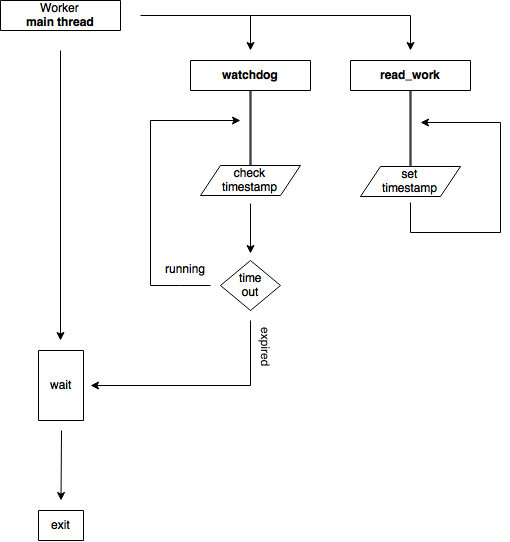
\includegraphics[width=\textwidth]{images/watchdog}
\caption{Schema della procedura di controllo sul tempo di esecuzione \label{fig: watchdog}}
\end{figure}
Il thread di \emph{watchdog}, letteralmente di sorveglianza, è adibito al controllo della \textbf{corretta esecuzione del worker},in particolare al controllo che tale esecuzione, nell'occupare per eccessivo tempo le risorse del sistema, non vado a creare un collo di bottiglia che via via porta al collasso del programma. Per far questo esso viene eseguito in modalità \emph{detached} dal thread principale del worker ed è legato dalle operazioni che vengono eseguite dal processo da una serie di variabili: 
\begin{itemize}
	\item \emph{pthread\_condition} su cui è in attesa il thread principale del worker
	\item \emph{flag} legata alla condition di cui sopra
	\item \emph{timestamp} settato dal thread di lettura della richiesta in arrivo
\end{itemize}
Come appare da una prima analisi della struct del watchdog.
\begin{lstlisting}
/*
 * ---------------------------------------------------------------------------
 * Structure        : typedef struct watchdog_thread
 * Description      : this struct helps to manage and set attributes for the thread
 *                    which watch over the remote connection thread termination
 * ---------------------------------------------------------------------------
 */
typedef struct watchdog_thread {
    int status;                                     
    pthread_cond_t *worker_await_cond;             
    int *worker_await_flag;

    time_t killer_time;                             // to schedule the watchdog wakeup
    time_t timeout_worker;                          // to abort a thread run
    time_t timestamp_worker;                        // timestamp last worker operation
} Watchdog, *WatchdogPtr;

\end{lstlisting}
Dove il \emph{killer\_time} ed il \emph{timeout\_worker} sono definiti dal file di configurazione per dare modo all'operatore di modellare l'implementazione sulle caratteristiche della macchina su cui gira il web switch. \\\\
Una più schematica rappresentazione del flusso di esecuzione è possibile vederla in \emph{\ref{fig: watchdog}}.
In particolare quando vengono distaccati i thread ausiliari, il thread principale del worker si mette in attesa della fine di una delle condizioni di termine del servizio di cui si è già discusso sopra, fra cui anche lo scadere del massimo tempo di esecuzione disponibile. In particolare, ad ogni iterazione del thread di lettura, avremo un aggiornamento del timestamp del worker, per cui ogni volta che si ha l'arrivo di una risposta da reinoltrare o di una richiesta da soddisfare si assume il server come operativo od il client in ascolto. \\ 
Contemporaneamente il watchdog rimane in \emph{nanosleep} per un lasso di tempo pari a quello configurato, a meno dell'arrivo di segnali che vengono gestiti e dopo i quali il watchdog ritorna in attesa, scaduto il quale la variabile di timestamp viene controllata. Se risulta \emph{scaduta} viene aggiornato il flag di attesa del worker e gli viene segnalato di riattivarsi e di mettere in pratica le procedure di \emph{clean up} per scollegarsi dal client e dal server assegnato. \\\\
Osserviamo come questo controllo viene fatto su una variabile settata dal thread di lettura, permettendoci con semplicità di valutare eventuali problemi sia sulla linea fra web switch e macchina del cluster che fra web switch e client, evitando lo stato di \emph{hanging} che porterebbe ad uno stallo del programma.
\newpage
\section{Ulteriori proposte}

\newpage
\section{Politiche di scheduling}
 \label{sec: sched_p}
La schedulazione permette la selezione della macchina predisposta a rispondere alla richiesta HTTP appena arrivata da parte del client, si basa su una tecnica nota come \textbf{bilanciamento del carico}, ovvero la distribuzione del carico, solitamente di elaborazione o di erogazione di uno specifico servizio, tra più server. Questo permette di poter \textbf{scalare} sulla potenza di calcolo del cluster dietro al web switch, lasciando che siano diverse macchine a rispondere a seconda di quella che è più veloce, più performante, oppure monitorando costantemente lo stato dei server e scegliendo quello meno sottoposto ad una pressione del carico di lavoro. Le macchine, specificando hostname ed indirizzi IP, sono date in un apposito file di configurazione.
\\
\\ 
Nella nostra implementazione \textbf{thread scheduler} si occupa di fornire,  ogni volta che viene invocato, una macchina selezionata secondo una delle due politiche che andremo ora a spiegare nel dettaglio.

\subsection{State-less: implementazione con Round-Robin}
L'algoritmo di scheduling Round-Robin (da adesso RR, \emph{n.d.r.}) è un algoritmo che agisce con prelazione distribuendo in maniera equa il lavoro, secondo una metrica stabilita in partenza. Vediamo quindi la struttura che si occupa di gestire la schedulazione tramite Round-Robin e che contiene le funzioni \emph{wrapper} alle strutture dati che garantiscono il suo corretto funzionamento.\\
\begin{lstlisting}
/*
 * ---------------------------------------------------------------------------
 * Structure        : typedef struct round_robin_struct
 * Description      : This struct represents a Round Robin discipline that can
 *                     be used also a stateful discipline with minimum overhead
 *                    (weighted mode enabled)
 * ---------------------------------------------------------------------------
 */
typedef struct round_robin_struct {
    CircularPtr circular;

    ThrowablePtr (*weight)(CircularPtr circular, Server *servers, int server_num);
    ThrowablePtr (*reset)(RRobinPtr rrobin, ServerPoolPtr pool, int server_num);
    Server *(*get_server)(CircularPtr circular);
}RRobin, *RRobinPtr;

\end{lstlisting}
\begin{figure}[b]
\centering
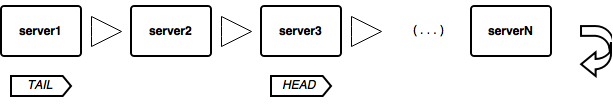
\includegraphics[width=\textwidth]{images/rrobin_stateless}
\caption{Schema di funzionamento del buffer circolare \label{fig: rrobin_sl}}
\end{figure}
Possiamo osservare come siano mantenuti i puntatori alle funzioni necessarie al caso di politica di scheduling \emph{state-aware}, ma per ora l'unica vera funziona a cui si farà accesso è quella per il recupero del server correntemente selezionato. \\\\
L'algoritmo funziona utilizzando un \textbf{buffer circolare} come possiamo vedere in \emph{figura \ref{fig: rrobin_sl}}: questo permette di iterare la selezione su una lista di elementi precedentemente caricata. Possiamo osservare che, oltre alle funzioni e le variabili necessarie a garantire l'accesso atomico all'area di memoria che contiene il buffer, necessario come vedremo nel caso \emph{state-aware} per evitare la concorrenza con il thread che si occupa dell'update dello stato, sono mantenuti:
	\begin{itemize}
  		\item Un puntatore all'array di server 
  		\item La posizione attuale del puntatore di \emph{testa} 
  		\item La lunghezza del buffer, necessaria anche per le operazioni di aggiornamento dei puntatori
  		\item I puntatori di \emph{testa} e \emph{coda} per avanzamento e lettura dal buffer
	\end{itemize}
	Le funzioni restanti permettono di inizializzare il buffer (oltre che di liberare con sicurezza l'area di memoria occupata) e di aggiornare i puntatori sopra menzionati.\\

\subsection{State-less: implementazione con Round-Robin}
L'algoritmo di scheduling Round-Robin (da adesso RR, \emph{n.d.r.}) è un algoritmo che agisce con prelazione distribuendo in maniera equa il lavoro, secondo una metrica stabilita in partenza.
\\
L'algoritmo funziona utilizzando un buffer circolare come possiamo vedere in \hyperref[fig: rrobin_sl]{\emph{figura}}: questo permette di iterare la selezione su una lista di elementi precedentemente caricata. E' necessario quindi specificare due passi per il corretto funzionamento, dopo aver dato un rapido sguardo alla struttura che lo rappresenta nella nostra implementazione.
\\
\\
\begin{lstlisting}
/*
 * ---------------------------------------------------------------------------
 * Structure        : typedef struct circular_buffer
 * Description      : This struct helps to manage a circular buffer of fixed length
 * ---------------------------------------------------------------------------
 */
typedef struct circular_buffer {
    Server      *buffer;
    int         buffer_position;
    int         buffer_len;
    
    Server      *head;
    Server      *tail;

    pthread_mutex_t mutex;

    ThrowablePtr (*allocate_buffer)(CircularPtr *circular, Server **servers, int len);
    ThrowablePtr (*acquire)(struct circular_buffer *circular);
    ThrowablePtr (*release)(struct circular_buffer *circular);
    void         (*progress)(struct circular_buffer *circular);
    void         (*destroy_buffer)(struct circular_buffer *circular);
} Circular, *CircularPtr;

\end{lstlisting}
\break
È necessario quindi specificare tre passi per il corretto funzionamento, dopo aver dato un rapido sguardo alla struttura che lo rappresenta nella nostra implementazione. \\\\
\textbf{Inizializzazione del buffer} in questa fase la struttura dati che rappresenta il buffer circolare, che abbiamo visto mantenere due puntatori di \emph{testa} e \emph{coda}, viene inizializzata associandovi un array di puntatori di strutture di tipo \emph{Server}, precedentemente allocata ed il cui pattern è stato fissato, e viene eseguita la funzione di allocazione del buffer: 
\begin{lstlisting}
    /* inside allocate_buffer ... */
    // allocating the buffer
    circular->buffer = *servers;
    circular->buffer_len = len;
    // setting params
    circular->head = circular->buffer;
    circular->tail = circular->buffer + (len - 1);
    
\end{lstlisting}
In un'ottica di \emph{produttore vs consumatore}, chiaramente visibile nella figura precedente, è necessario che testa e coda non coincidano mai per evitare concorrenza. In questa implementazione si è deciso di separare l'accesso concorrente alla struttura, per il suo aggiornamento, e la lettura dei dati in essa contenuti. Quindi la \emph{testa} conterrà il puntatore al prossimo server da selezionare per schedulare la richiesta, mentre la \emph{coda} punterà all'area di memoria contenente il server attualmente selezione per la schedulazione. \\\\
\textbf{Aggiornamento dei puntatori} per poter sfruttare le peculiarità di questa struttura dati è necessario che i due puntatori vengano aggiornati secondo l'aritmetica del buffer circolare per cui, una volta raggiunta l'estremità dell'array, il valore successivo della posizione corrente ritorna ad essere quello del primo valore dello stesso array. \\
Nel dettaglio viene eseguito, secondo le specifiche sopra riportate, nella nostra implementazione, la seguente funzione:
\begin{lstlisting}
void progress(CircularPtr circular) {
    // recomputing tail, head and buffer position
    circular->tail            = circular->head;
    circular->buffer_position = (circular->buffer_position + 1) % circular->buffer_len;
    circular->head            = circular->buffer + circular->buffer_position;
}

\end{lstlisting}
\textbf{Selezione del server} a questo punto, una volta che il thread chiamante invoca lo scheduler per recuperare il server che è stato selezionato dall'algoritmo, lo scheduler a sua volta invoca la funzione wrapper dalla struttura che gestisce la politica RR e questa esegue il codice ora riportato.
\begin{lstlisting}
    /* inside get_server ... */
    // allocating server ready struct
    ServerPtr server_ready = malloc(sizeof(Server));
   
    /* ... */
    
    // stepping the circular buffer
    circular->progress(circular),
    // retrieving server from tail 
    *server_ready = *(circular->tail);
    return server_ready;
    
\end{lstlisting}
In conclusione quello che stiamo attuando è un \textbf{bilanciamento del carico uniforme} su ognuna delle macchine del cluster. Infatti, senza condizioni sullo stato delle macchine, iterando semplicemente sull'array dei server, ad ogni nuova connessione verrà assegnata una macchina diversa, alleggerendo tutti i server e pareggiando per ciascuno il carico. Il cluster manterrà il carico complessivo ma ogni singola unità contribuirà equamente a soddisfare le connessioni in arrivo.
\newpage
\subsection{State-aware: implementazione con monitor di carico}

\begin{figure}[t]
\centering
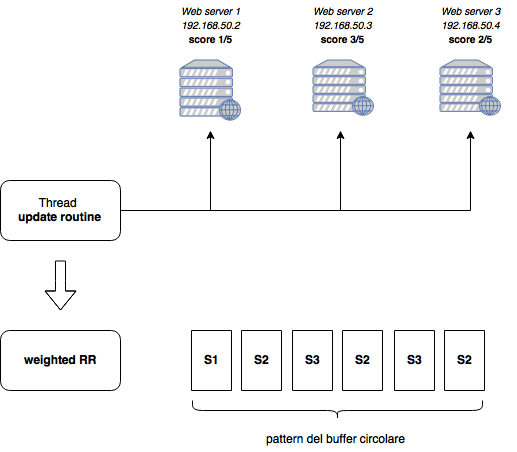
\includegraphics[width=\textwidth]{images/rrobin_stateaware}
\caption{Schema della procedura di aggiornamento dello stato dei server 
\label{fig:rrobin_sa}}
\end{figure}

Un algoritmo di schedulazione cosiddetto \emph{state-aware} si occupa di selezionare la macchina a cui inoltrare la connessione basandosi non solo sulla conoscenza delle macchine presenti nel cluster ma anche sul loro status. In particolare, in questa implementazione, si è deciso di ricorrere all'analisi dei risultati di un \textbf{monitor di carico} presente su ciascuna delle macchine del cluster (in riferimento alle assunzioni progettuali, questi è i modulo \emph{ApacheStatus} di cui si parlerà più avanti in \emph{\ref{sssec:apachestatus}} ). Tale monitor, che ritorna una serie di parametri indici dell'attuale impiego di risorse della macchina, permette di definire un \textbf{algoritmo pesato} per la selezione del server che risponderà alla connessione in arrivo al web switch. \\
Anche in questo caso andremo a determinare una serie di passi che vengono seguiti, tenendo conto che in fase progettuale \emph{si è deciso di sfruttare lo stesso algoritmo RR} già utilizzato nel caso \emph{state-less}, ma che ricordiamo essere stato predisposto per una ulteriore versione pesata. Per far questo si lavora sulla struttura Server \\\\
\textbf{Detachment del thread di update} nei file di configurazione dell'applicazione è possibile definire due livelli di lavoro:
	\begin{itemize}
		\item \textbf{AWARENESS\_LEVEL\_LOW} che corrisponde ad una versione state-less dell'algoritmo RR e si riporta al caso precedente
		\item \textbf{AWARENESS\_LEVEL\_HIGH} che corrisponde all'algoritmo state-aware e che necessiterà di una routine di aggiornamento dello stato delle macchine del cluster
	\end{itemize}
	Il secondo caso è proprio quello qui descritto e corrisponde a lavorare utilizzando, oltre al thread principale che si occupa di accettare le connessioni in arrivo, un \textbf{thread predisposto alla sola verifica dello stato dei server}. Tale thread viene istanziato nel momento in cui viene inizializzato lo scheduler e vengono allocate le strutture dati alla base di RR. \\
	Il lavoro di tale thread, che ora vedremo nel dettaglio, è quello deducibile da \emph{figura \ref{fig:rrobin_sa}}.\\\\
\textbf{Routine di score} all'interno di questa routine, che viene eseguita da un thread distaccato e che viene eseguita una volta ogni \emph{UP\_TIME} secondi, tempo di update in secondi definito dall'utente nei file di configurazione, viene richiamata più volte la funzione che si occupa di recuperare e parsare l'interrogazione del modulo \emph{ApacheStatus} e recupare da questa i \textbf{worker in \emph{idle state} ed i worker in \emph{busy state}}. A questo punto si va a modificare il nodo della pool dei server precedentemente allocata (di cui si è già parlato in \emph{\ref{ssec: sched}}). Viene quindi eseguita la sequente routine. \\
\begin{lstlisting}
    /* inside apache_score ... */
    // retrieving status from remote Apache machine
    throwable = apache_status->retrieve(apache_status);   
    //checking for errors or if server is currently down
    if (throwable->is_an_error(throwable)) {
        server->weight = WEIGHT_DEFAULT;
        server->status = SERVER_STATUS_BROKEN;
        return throwable->thrown(throwable, "apache_score");
    } else {
        server->status = SERVER_STATUS_READY;
    }
    
    /* ... */
    int score;
    int IDLE_WORKERS  = apache_status->idle_workers;
    int TOTAL_WORKERS = apache_status->busy_workers + IDLE_WORKERS;

    // calculating and setting score - mapping in [w, W]
    score = (IDLE_WORKERS   - WEIGHT_DEFAULT)   *
            (WEIGHT_MAXIMUM - WEIGHT_DEFAULT)   /
            (TOTAL_WORKERS  - WEIGHT_DEFAULT)   +   WEIGHT_DEFAULT;
    server->weight = score;
       
\end{lstlisting}
Alla fine quello che ottengo è uno \textbf{score} che vado a settare nel nodo contenuto nella \textbf{pool dei server} che viene definito dalla relazione matematica che è così esplicitata:
\begin{align*}
	score\Big(\frac{IDLE\_WORKERS}{TOTAL\_WORKERS}\Big) ~ \in ~ [w, W]
\end{align*}
ottenendo quello che un \emph{mapping} del rapporto fra i worker occupati nella macchina ed i worker totali a disposizione di Apache per rispondere ad una richiesta in arriva. Tale indice viene memorizzato come \emph{peso del server nel cluster}.\\
Notiamo che nel caso ci siano problemi nel recuperare l'indice di score si supporrà che il server non è momentaneamente disponibile ed il suo status verrà segnalato come BROKEN, fino al prossimo aggiornamento.\\\\
\textbf{RR pesato} dai nodi della pool dei server aggiornati con il loro peso viene costruito, secondo lo schema in \emph{\ref{fig:rrobin_sa}}, un pattern dei server secondo il loro peso, di modo da distribuire il carico secondo sempre un algoritmo RR, ma in cui per ogni sequenza il server viene selezionato un numero di volte pari al suo peso: comparirà massimo \emph{W} in caso di basso carico di lavoro ed al minimo \emph{w} volte in condizioni di forte stress. I due parametri sono, in questa implementazione, macro che possono essere modificate a seconda dei limiti delle macchine del proprio cluster, di default \emph{w = 1} e \emph{W = 5}, soggetti al tuning del web switch in fase di installazione ed ottimizzazione. Alla prima iterazione tutte le macchine so di default settata con peso minimo (pari a \emph{w})\\\\ 
In conclusione, con questa opzione abilitata, si ha la possibilità di ridistribuire equamente il lavoro, permettendo al web switch di adattare la distribuzione del carico a secondo dello stato attuale, evitando di sovraccaricare nodi sensibili allo stress in determinate condizioni o che sono stati sottoposti già ad uno stress eccessivo. Si è scelto di riadattare RR per ottenere una soluzione modulare e che fosse facile riadattare ed ottimizzare a seconda di entrambe le condizioni operative, sia senza che con conoscenza dello stato delle macchine. Osserviamo infatti che in entrambi i casi RR risulta pesato, nel secondo caso preso in esame tale peso non è più fisso e minimo ma variabile dipendentemente dalle condizioni delle macchine.\\\\
La ricerca di una soluzione modulare che possa essere presa poi in esame da futuri sviluppatore e possa essere oggetto di un \emph{tuning} più approfondito, è stata intrapresa perseguendo il principio per cui \emph{simplicity favours regularity}.

\subsubsection{Modulo Apache Status}
\label{sssec:apachestatus}
Il modulo Apache Status (modstatus) è un modulo che fornisce informazioni sull'attività e le prestazioni del server in cui è installato. Questo modulo è disponibile nella versione base di Apache senza il bisogno di dover scaricare nient altro, per utilizzarlo è necessario solo attivarlo nella configurazione del sito. Il modulo formatta tramite una pagina HTML tutta una serie statistiche e dati facilmente leggibili da un essere umano (oppure nella sua variante machine readble che in questa applicazione usiamo). I dettagli che fornisce sono il numero di worker che servono richieste, il numero di worker che sono in pausa, lo stato di ognuno di questi worker, il numero di accessi e byte serviti, il numero di richieste per secondo e la percentuale di CPU usata da ogni worker e in totale da Apache.
Tramite questo modulo quindi siamo stati in grado di poter verificare lo stato di una macchina senza la necessità di installare nessun componente aggiuntivo.


\newpage
\section{Logging}
\newpage
\section{Performance}
\subsection{Test di carico}
\subsection{Comparazione con Apache}
\newpage
\section{Future implementazioni}
\subsection{Analisi della richiesta}
\subsection{Webserver performante}


% --- References ---  
%
% bibtex is used to generate the bibliography. The babplain style
% will generate numeric references (e.g. [1]) appropriate for theoretical
% computer science. If you need alphanumeric references (e.g [Tur90]), use
%
% \bibliographystyle{babalpha-lf}
%
% instead.


\newpage
%\bibliographystyle{babplain-lf}
%\bibliography{references}
\renewcommand{\refname}{\normalfont\selectfont\normalsize\textbf{Annotazioni}} 
\begin{thebibliography}{9}
\bibitem{lamport94}
  Leslie Lamport,
  \emph{\LaTeX: a document preparation system},
  Addison Wesley, Massachusetts,
  2nd edition,
  1994.
  
\end{thebibliography}

% --- Appendices --- 
\newpage
\appendix
 
\section{Manuale per l'uso}

\section{Vagrant}

Durante lo sviluppo ci siamo imbattuti in alcune problematiche
legate alla portabilità del codice che stavamo scrivendo, errori di inclusione di file header, funzioni con comportamenti anomali, macro differenti e problemi nella compilazione. Questo perché lo sviluppo procedeva su macchine con sistemi operativi differenti, nello specifico Mac OSX e Debian. Da qui la necessità di avere un ambiente unificato per l'esecuzione del codice. La soluzione al problema era di facile intuizione, creare una macchina virtuale su VirtualBox e distribuirla su tutti i computer utilizzati per lo sviluppo, purtroppo però mettere in piedi questa soluzione può rivelarsi un'operazione tediosa, installazione del sistema operativo, configurazione dei programmi per lo sviluppo e condivisione di una VM che pesa diversi MB.\\\\
\textbf{Vagrant} è uno strumento per la creazione di ambienti di sviluppo completo. Fondamentalmente si tratta di un’applicativo scritto in Ruby che sfruttando le API messe a disposizione da VirtualBox è in grado di manipolare la gestione delle macchine virtuali al suo interno. Il tutto semplicemente compilando una "ricetta" chiamata Vagrantfile. Il \textbf{Vagrantfile} è un file all’interno del quale si inseriscono tutte le specifiche riguardo la VM che vogliamo preparare, impostando il sistema operativo, ulteriori programmi da installare, cartelle condivise, configurazioni di rete e quant'altro. Una volta preparato il vagrantfile questo può essere condiviso tra tutti gli sviluppatori, quindi senza dover condividere l'intera VM basterà solo questo file per poter avere tutte le macchine virtuali allo stesso stato. Ogni volta che uno sviluppatore avrà necessità di modificare il comportamento della VM basterà modificare il Vagrantfile e condividerlo con gli altri. Ultima caratteristica è che vagrant è pensato per lasciare allo sviluppatore la scelta dell'IDE che preferisce creando un ambiente completamente trasparente per lo sviluppo del software.\\\\
\emph{Vagrant makes the "works on my machine" excuse a relic of the past.}

\section{Cluster virtuale}

\section{Tool per i debug}
\subsection{GDB}
\subsection{Valgrind}

\section{Tool per i test}
\subsection{PostMan}
\subsection{Telnet}
\subsection{HttPerf}
\subsection{Browser}

\end{document}